% System Design of \chameleon{}

%%%%%%%%%%%%%%%
\begin{frame}{}
  \begin{center}
    \chameleon{} prototype: \\[10pt]
    A prototype \textbf{partitioned} \textbf{replicated} \\[6pt]
    distributed transactional \textbf{key-value} store
  \end{center}
\end{frame}
%%%%%%%%%%%%%%%

%%%%%%%%%%%%%%%
\begin{frame}{}
  \begin{center}
    Classic \textbf{key-value} data model \\[4pt]
      Key: (row key, column key)
  \end{center}
\end{frame}
%%%%%%%%%%%%%%%

%%%%%%%%%%%%%%%
\begin{frame}{}
  % \fignocaption{width = 0.70\textwidth}{figs/chameleon-arch.pdf}
  \begin{center}
    \resizebox{0.70\textwidth}{!}{%        File: chameleon-arch.tex
%     Created: Mon Jan 04 08:00 PM 2016 C
% Last Change: Mon Jan 04 08:00 PM 2016 C
% 	    Used in Beamer

\begin{tikzpicture}[connection/.style = {>=Stealth, <->, brown, dashed, line width = 3pt}]
  % background: china map
  \node (china-map) [opacity = 0.20] {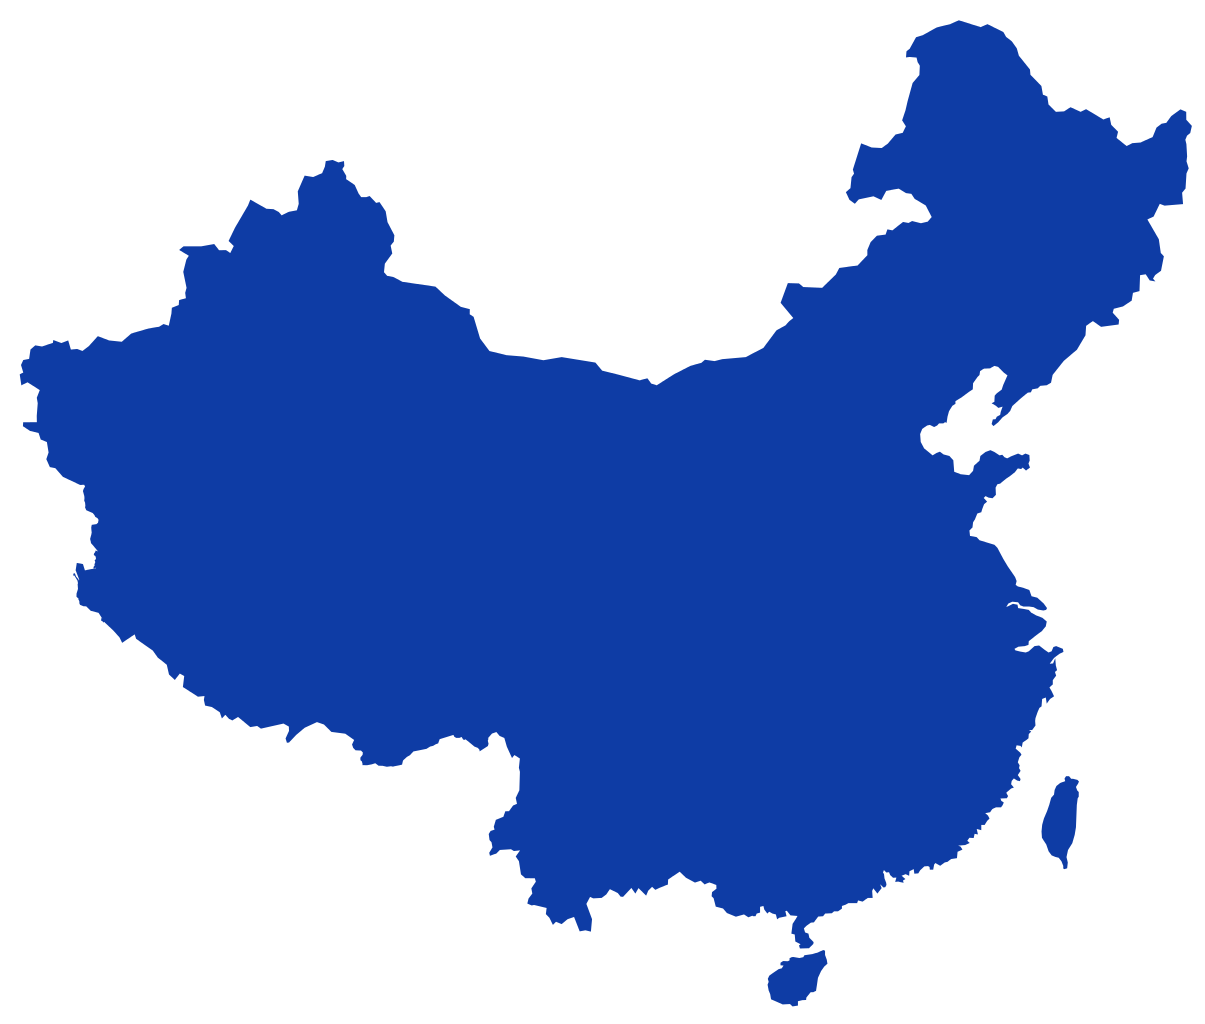
\includegraphics[scale = 0.40]{figs/china-outline-blue.png}};

  % partition-left, partition-right, partition-below
  \uncover<2->{
    \node (partition-left) [] at (-6.5, 1) {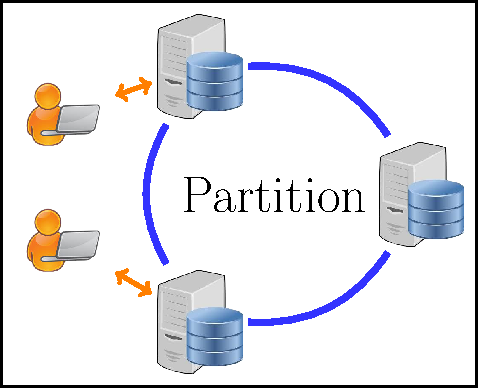
\includegraphics[scale = 0.80]{figs/partition.pdf}}; 
  }
  \uncover<3->{
    \node (partition-right) [] at (6, 3.5) {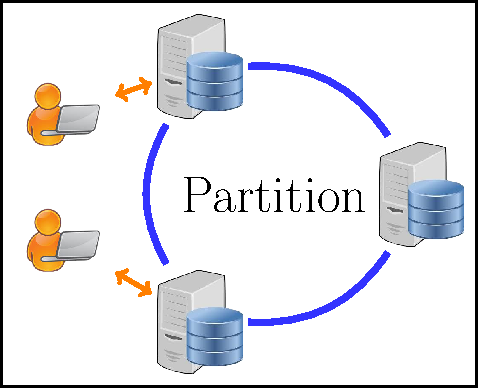
\includegraphics[scale = 0.80]{figs/partition.pdf}}; 
    \node (partition-below) [] at (1.5, -5) {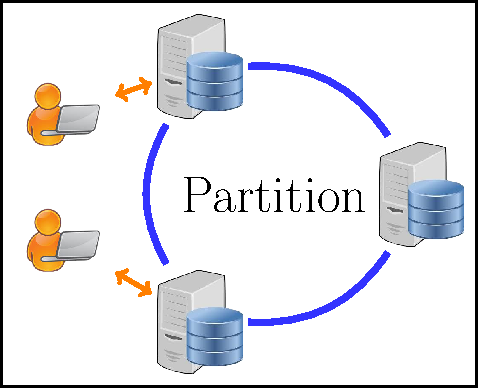
\includegraphics[scale = 0.80]{figs/partition.pdf}}; 

    % connections among partitions
    \draw [connection] (partition-left) to (partition-right); 
    \draw [connection] (partition-right) to (partition-below);
    \draw [connection] (partition-below) to (partition-left);

    % replication 
    \node (replication) [font = \Huge, align = center] at (0.5, 0.0) {\textbf{Wide-area}\\[3pt]\textbf{Replication}};
  }

  \uncover<4->{
    % master-slave for one partition
    \begin{scope}[circled/.style = {draw, circle, dash pattern = on 10pt off 5pt, cyan, line width = 2pt, outer sep = 5pt, minimum size = 2.0cm}, 
      conn/.style = {dash pattern = on 15pt off 8pt, cyan, line width = 2pt}]
    \node (ms-left) [circled] at (-4., 1) {};
    \node (ms-right) [circled] at (5.5, 1.7) {};
    \node (ms-below) [circled] at (4., -5.0) {};

    \node (master-slave) [below right = 1.5cm and -1.5cm of partition-right] {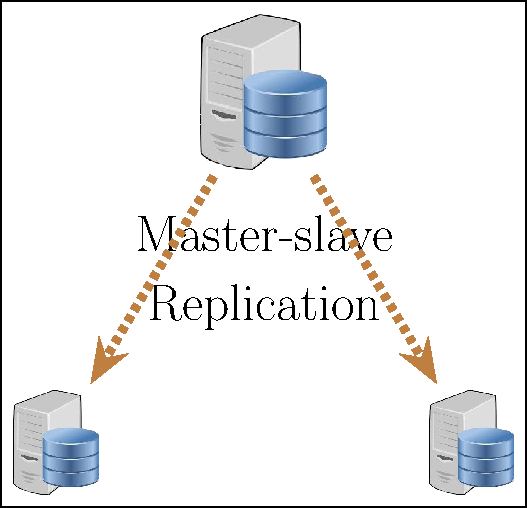
\includegraphics[scale = 0.80]{figs/master-slave.pdf}};
    \draw [conn] (ms-left) to (master-slave);
    \draw [conn] (ms-right) to (master-slave);
    \draw [conn] (ms-below) to (master-slave);
    \end{scope}
  }
\end{tikzpicture}
}
  \end{center}

  \begin{center}
    \only<2>{Keys are \textbf{partitioned} within a single datacenter.}
    \only<3-4>{Each key is \textbf{replicated} across datacenters} \only<4>{in a \textbf{master-slave} manner.}
    \only<5>{Transactions are first executed and committed on the \textbf{masters},\\
      and are then asynchronously propagated to \textbf{slaves}.}
  \end{center}
\end{frame}
%%%%%%%%%%%%%%%

%%%%%%%%%%%%%%%
\begin{frame}{}
  \only<1-3, 5->{\fignocaption{width = 0.50\textwidth}{figs/chameleon-framework.pdf}}

  \begin{center}
    \only<2>{\blue{1.} Partitioned replicated transactional key-value store}
    \only<3>{\blue{2.} Client library}
    \only<5>{\blue{3.} \rvsi{} protocol: \rvsims{} + \rvsimp{}}
  \end{center}

  \only<4>{
    \centerline{Code snippet for writing \rvsi{} transactions:}
    \vspace{0.30cm}
    \begin{lstlisting}[
  language = Java,
  basicstyle = \ttfamily\footnotesize,
  showstringspaces = false,
  keywordstyle = \color{blue}\bfseries,
  commentstyle = \color{teal},
  stringstyle = \bfseries,
  upquote = true,
  frame = box,
  breaklines = true,
  linewidth = 0.85\textwidth
]
  // Initialize keys (ck, ck1, and ck2) here
  ITx tx = new RVSITx(/** context **/);

  tx.begin();

  // Read and write
  ITsCell tsCell = tx.read(ck);
  ITsCell tsCell1 = tx.read(ck1);
  tx.write(ck1, new Cell("R1C1"));
  ITsCell tsCell2 = tx.read(ck2);

  // Specify RVSI specs. (e.g., SVSpec)
  RVSISpec sv = new SVSpec();
  sv.addSpec({ck, ck1, ck2}, 2);
  tx.collectRVSISpec(sv);

  boolean committed = tx.end();
\end{lstlisting}

  }
\end{frame}
%%%%%%%%%%%%%%%
